\documentclass[12pt,a4paper]{article}
\usepackage[utf8]{inputenc}
\usepackage[T2A]{fontenc}
\usepackage[russian]{babel}
\usepackage{graphicx}
\usepackage{booktabs}
\usepackage{longtable}
\usepackage{geometry}
\usepackage{float}
\geometry{top=2cm, left=2cm, right=2cm, bottom=2cm}
\usepackage{paracol}
\usepackage{src/title}
\usepackage{hyperref}
\usepackage{listings}
\usepackage{xcolor}

\title{Лабораторная работа 3. Линейная регрессия на данных о жилье Калифорнии}
\author{Ануфриев А.С. 465029}
\supervisor{Болдырева Е. А.}
\date{07.11.2026}

\abstract{
В работе выполнен анализ датасета о жилье в Калифорнии (17~000 записей, 9 признаков). Получена описательная статистика, проведена предобработка данных, реализована линейная регрессия методом наименьших квадратов собственным кодом на языке Python с использованием NumPy. Построены и сравнены три модели с разными наборами признаков по коэффициенту детерминации R$^2$, введен синтетический признак. Результаты оформлены в виде отчёта с графиками и таблицами.
}
\keywords{линейная регрессия, метод наименьших квадратов, коэффициент детерминации, данные о жилье, Python, NumPy}

\begin{document}
\maketitle

\section{Цели и задачи}
Цель работы --- построение и сравнение моделей линейной регрессии для прогнозирования стоимости жилья в Калифорнии методом наименьших квадратов без применения готовых библиотек регрессии. Основные задачи:
\begin{enumerate}
\item получить и визуализировать описательную статистику по датасету (количество, среднее, стандартное отклонение, минимум, максимум, квантили);
\item выполнить предобработку данных: обработку отсутствующих значений, кодирование категориальных признаков, нормировку;
\item разделить данные на обучающую и тестовую выборки;
\item реализовать линейную регрессию методом наименьших квадратов собственным кодом (минимизация суммы квадратов разностей фактических и предсказанных значений), используя только NumPy и Pandas;
\item построить три модели с разными наборами признаков;
\item оценить каждую модель коэффициентом детерминации R$^2$ и сравнить результаты;
\item в качестве бонуса ввести синтетический признак.
\end{enumerate}

\section{Теоретические сведения}
Линейная мультимножественная регрессия описывает зависимость результативного признака $y$ от нескольких факторов $x_1,\dots,x_p$:
\begin{equation}
\hat{y} = a + b_1 x_1 + \dots + b_p x_p .
\end{equation}
Метод наименьших квадратов определяет оценки параметров вектором $B = (a,b_1,\dots,b_p)^\top$ как
\begin{equation}
B = (X^\top X)^{-1} X^\top Y ,
\end{equation}
где $X$ --- матрица признаков с первым столбцом единиц (свободный член), $Y$ --- вектор наблюдений целевой переменной. Качество модели оценивается коэффициентом детерминации
\begin{equation}
R^2 = 1 - \frac{\sum_i (y_i - \hat{y}_i)^2}{\sum_i (y_i - \bar{y})^2} .
\end{equation}

\section{Исходные данные}
Исходный датасет содержит 17~000 записей о жилых районах Калифорнии. Все 9 признаков числовые, пропущенных значений и категориальных признаков в исходных данных отсутствуют. Целевая переменная --- $median\_house\_value$ (медианная стоимость дома, тыс. долл.). Ограничение исходных данных: значения стоимости ограничены сверху отметкой 500 000 (цenzурное отсечение); записей на этой границе всего 22 (0,13 %), и доход у них разный, поэтому это не выброс, подлежащий удалению, а техническая особенность датасета.

\section{Ход работы}
\subsection{Загрузка данных и описательная статистика}
Данные загружены из CSV-файла. Вычислены размер выборки, среднее значение, стандартное отклонение, минимум, максимум и квантили 25\%, 50\%, 75\% для всех признаков (таблица~\ref{tab:stats}).

\begin{table}[H]
\centering
\caption{Описательная статистика по датасету.}
\label{tab:stats}
\small
\begin{tabular}{lrrrrrrrr}
\toprule
Признак & count & mean & std & min & 25\% & 50\% & 75\% & max \\
\midrule
longitude & 17000 & -119.56 & 2.01 & -124.35 & -121.79 & -118.49 & -118.00 & -114.31 \\
latitude & 17000 & 35.63 & 2.14 & 32.54 & 33.93 & 34.25 & 37.72 & 41.95 \\
housing\_median\_age & 17000 & 28.59 & 12.59 & 1.0 & 18.0 & 29.0 & 37.0 & 52.0 \\
total\_rooms & 17000 & 2643.66 & 2179.95 & 2.0 & 1462.0 & 2127.0 & 3151.25 & 37937.0 \\
total\_bedrooms & 17000 & 539.41 & 421.50 & 1.0 & 297.0 & 434.0 & 648.25 & 6445.0 \\
population & 17000 & 1429.57 & 1147.85 & 3.0 & 790.0 & 1167.0 & 1721.0 & 35682.0 \\
households & 17000 & 501.22 & 384.52 & 1.0 & 282.0 & 409.0 & 605.25 & 6082.0 \\
median\_income & 17000 & 3.88 & 1.91 & 0.50 & 2.57 & 3.54 & 4.77 & 15.00 \\
median\_house\_value & 17000 & 207300.91 & 115983.76 & 14999.0 & 119400.0 & 180400.0 & 265000.0 & 500001.0 \\
\bottomrule
\end{tabular}
\end{table}

Для целевой переменной построена гистограмма распределения (рисунок~\ref{fig:hist}), для пары ``доход населения --- стоимость жилья'' --- диаграмма рассеяния (рисунок~\ref{fig:scatter}).

\begin{figure}[H]
\centering
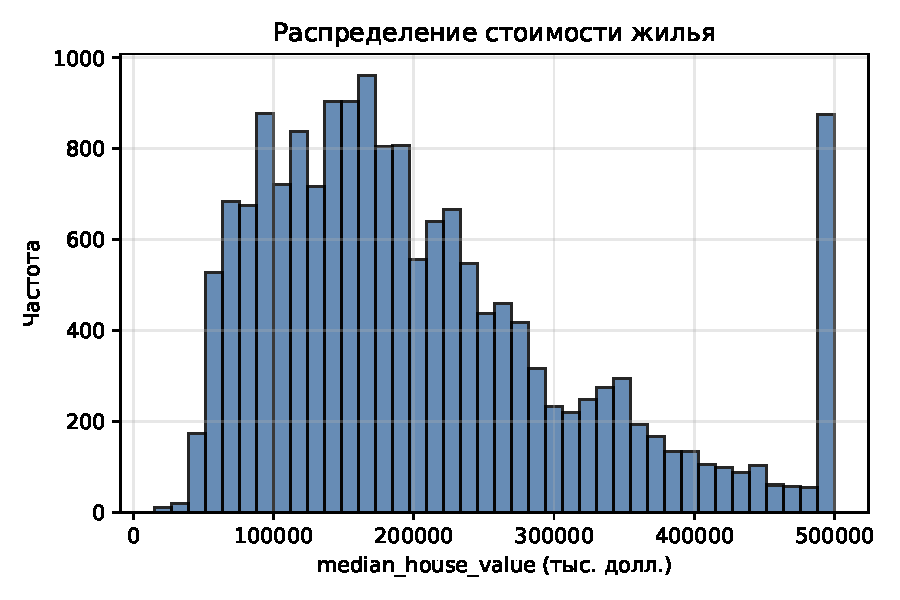
\includegraphics[width=0.55\linewidth]{../graphics/target_hist.pdf}
\caption{Гистограмма распределения медианной стоимости жилья.}
\label{fig:hist}
\end{figure}

\begin{figure}[H]
\centering
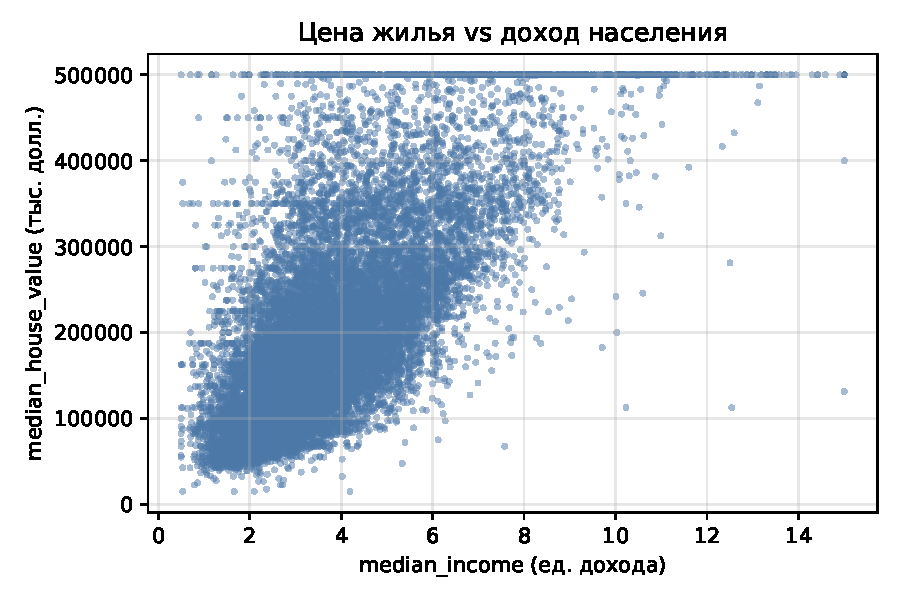
\includegraphics[width=0.55\linewidth]{../graphics/price_vs_income.pdf}
\caption{Диаграмма рассеяния стоимости жилья от дохода населения.}
\label{fig:scatter}
\end{figure}

\subsection{Предобработка данных}
Пропущенных значений в данных не обнаружено, категориальных признаков нет. Все числовые признаки нормированы стандартизацией (вычет среднего, деление на стандартное отклонение); целевая переменная не нормировалась.

\subsection{Разделение на выборки}
Данные перемешаны и разделены на обучающую (13~600 записей, 80\%) и тестовую (3~400 записей, 20\%) выборки.

\subsection{Реализация линейной регрессии}
Коэффициенты регрессии вычислены собственным кодом на языке Python с использованием NumPy по формуле $B=(X^\top X)^{-1}X^\top Y$, что эквивалентно минимизации суммы квадратов разностей фактических и предсказанных значений. Готовые средства регрессии не использовались.

\subsection{Три модели и синтетический признак}
Построены три модели с разными наборами признаков (таблица~\ref{tab:models}). В третью модель включён синтетический признак $rooms\_per\_household = total\_rooms / households$ (бонусное задание).

\begin{table}[H]
\centering
\caption{Сравнение трёх моделей линейной регрессии (признаки нормированы).}
\label{tab:models}
\small
\begin{tabular}{lll}
\toprule
Модель & Признаки & $R^2$ на тестовой выборке \\
\midrule
Модель 1 & median\_income & 0.4978 \\
Модель 2 & median\_income, housing\_median\_age & 0.5376 \\
Модель 3 & median\_income, total\_rooms, households, rooms\_per\_household & 0.5227 \\
\bottomrule
\end{tabular}
\end{table}

Оценочные коэффициенты моделей (включая свободный член, для нормированных признаков):
\begin{center}
\small
\begin{tabular}{lrrrr}
\toprule
& Модель 1 & Модель 2 & Модель 3 \\
\midrule
Свободный член & 207066.73 & 206962.89 & 207033.39 \\
median\_income & 79512.76 & 81929.71 & 89613.01 \\
housing\_median\_age & --- & 21519.53 & --- \\
total\_rooms & --- & --- & -54374.09 \\
households & --- & --- & 56290.68 \\
rooms\_per\_household & --- & --- & -6.13 \\
\bottomrule
\end{tabular}
\end{center}

\begin{figure}[H]
\centering
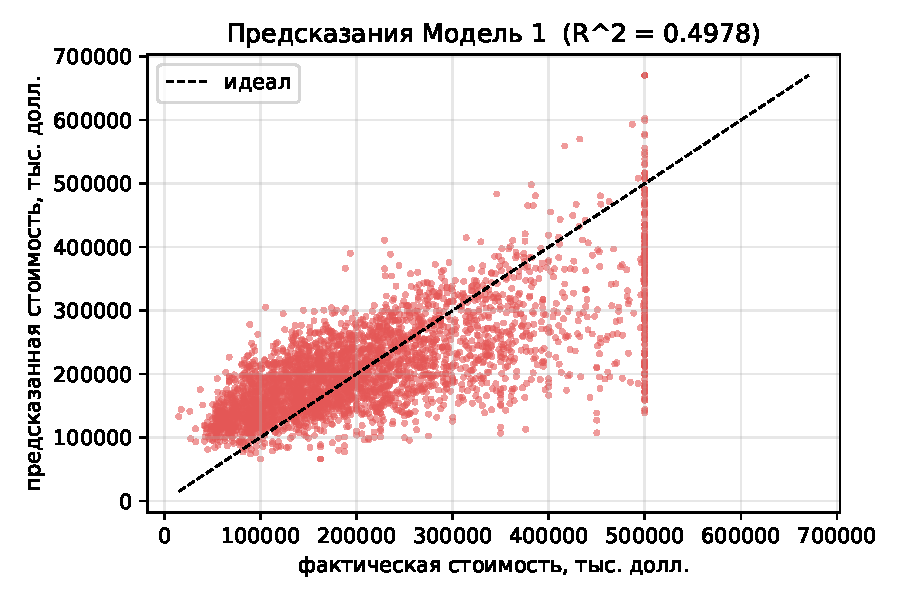
\includegraphics[width=0.5\linewidth]{../graphics/pred_1.pdf}
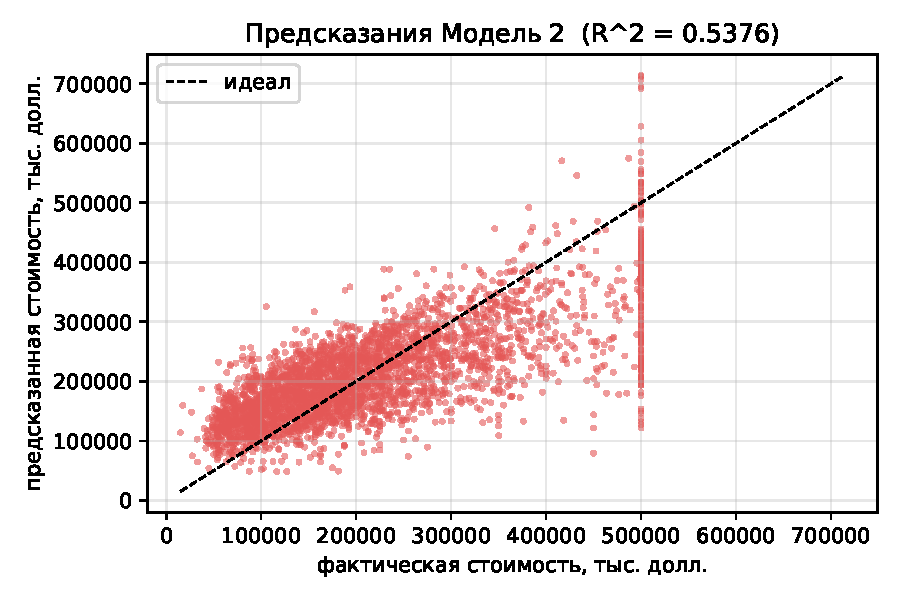
\includegraphics[width=0.5\linewidth]{../graphics/pred_2.pdf}
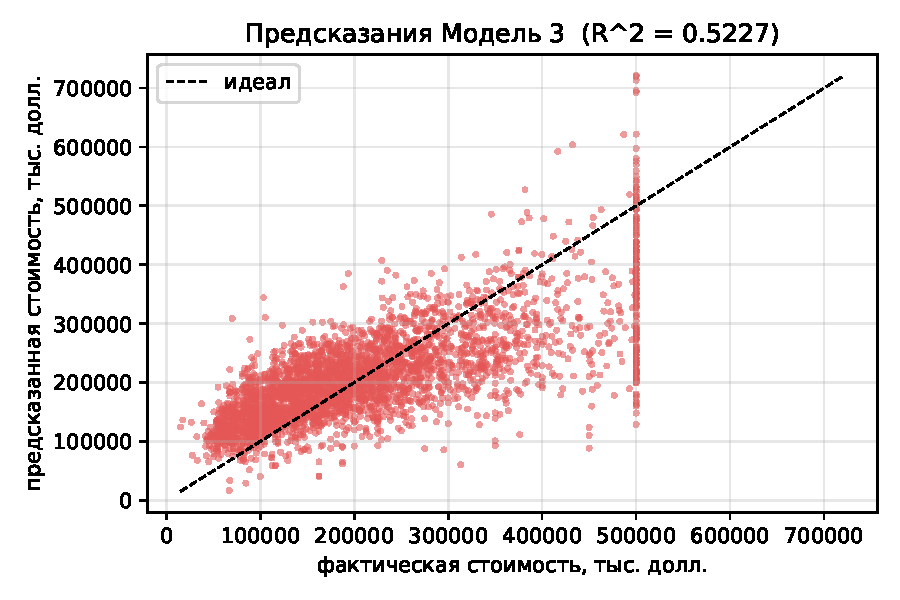
\includegraphics[width=0.5\linewidth]{../graphics/pred_3.pdf}
\caption{Фактические против предсказанных значений на тестовой выборке для моделей 1, 2 и 3.}
\label{fig:pred}
\end{figure}

\section{Выводы}
Наилучшее качество среди трёх моделей показала Модель 2 (признаки: доход населения и возраст жилого дома), $R^2 \approx 0.54$ на тестовой выборке. Доход населения является сильнейшим отдельным признаком ($R^2 \approx 0.50$ в одномерной модели). Добавление возраста дома повысило качество, а добавление в третью модель количества комнат, числа домохозяйств и синтетического признака не улучшило её ($R^2 \approx 0.52$), что связано с сильной линейной зависимостью (мультиколлинеарностью) между количеством комнат, числом домохозяйств и отношением комнат к домохозяйствам. Синтетический признак не дал преимущества при одновременном включении с его исходными компонентами.

\section{Приложение}
Минимальный фрагмент реализации метода наименьших квадратов (NumPy):
\begin{lstlisting}[language=Python, basicstyle=\footnotesize\ttfamily]
X_aug = np.column_stack([np.ones(len(X)), X])
B = np.linalg.inv(X_aug.T @ X_aug) @ X_aug.T @ y
y_pred = X_aug_test @ B
R2 = 1 - np.sum((y_true - y_pred)**2) / np.sum((y_true - y_true.mean())**2)
\end{lstlisting}
Полная реализация: скрипт расчётов, формирующий статистику, три модели, метрики $R^2$ и исходные данные для графиков.

\end{document}
